\section{Anhang}

\subsection{Wie löst man WrStat Übungen?}

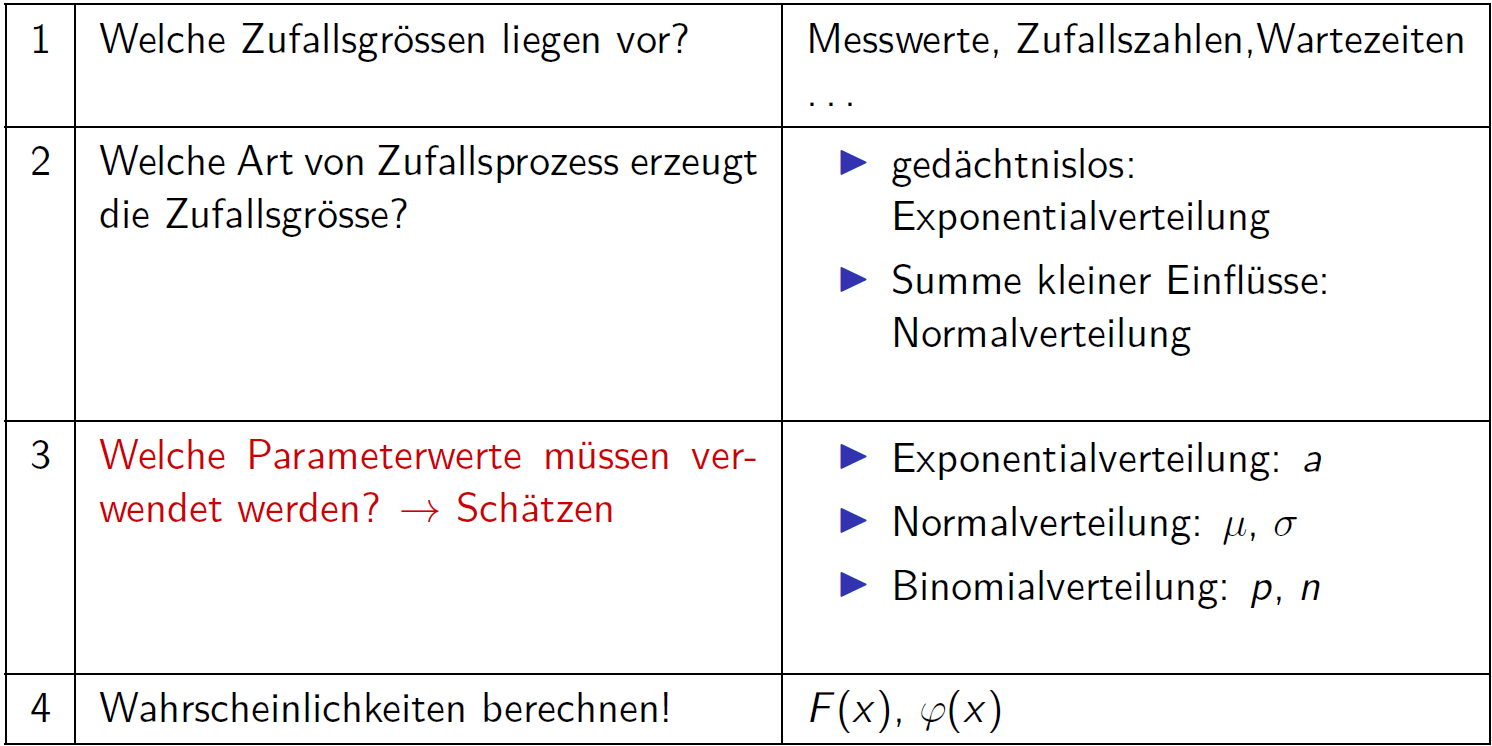
\includegraphics[width=\columnwidth]{images/wrstat_uebungen_loesen.png}

\subsection{Berechnungsformular}

\renewcommand{\arraystretch}{1.5}
\setlength{\tabcolsep}{3pt}
\begin{minipage}[c]{0.56\columnwidth}
\resizebox{\linewidth}{!}{%
\begin{tabular}{|c|c|c|c|c|c|}
    \hline
    $i$ & $x_i$ & $y_i$ & $x_i^2$ & $y_i^2$ & $x_i y_i$ \\ \hline
    $1$ & & & & & \\
    $2$ & & & & & \\
    $\vdots$ & & & & & \\
    $n$ & & & & & \\ \hline
    \color{gray}$\sum$ & \color{gray}$\sum x_i$ & \color{gray}$\sum y_i$ & \color{gray}$\sum x_i^2$ & \color{gray}$\sum y_i^2$ & \color{gray}$\sum x_i y_i$ \\ \hline
    \crd{$\cdot \frac{1}{n}$} & \color{gray}$E(X)$ & \color{gray}$E(Y)$ & \color{gray}$E(X^2)$ & \color{gray}$E(Y^2)$ & \color{gray}$E(XY)$ \\ \hline
\end{tabular}}
\end{minipage}
\hfill
\begin{minipage}[c]{0.42\columnwidth}
\resizebox{\linewidth}{!}{%
\begin{tabular}{|l|l|}
    \hline
    $\var(X)$       & \color{gray}$= E(X^2) - E(X)^2$ \\
    $\var(Y)$       & \color{gray}$= E(Y^2) - E(Y)^2$ \\
    $\cov(X, Y)$    & \color{gray}$= E(XY) - E(X)\,E(Y)$ \\ \hline
    $a$             & \color{gray}$= \cov(X, Y) / \var(X)$ \\
    $b$             & \color{gray}$= E(Y) - a\,E(X)$ \\ \hline
    $r$             & \color{gray}$= \dfrac{\cov(X, Y)}{\sqrt{\var(X) \, \var(Y)}}$ \\[0.8em] \hline
\end{tabular}}
\end{minipage}
\renewcommand{\arraystretch}{1}
\setlength{\tabcolsep}{6pt}

\smallskip
{\small \crd{Achtung:} $E(\ldots) = \frac{1}{n} \sum_{i=1}^{n} \ldots$ \; (Spaltensumme \textbf{geteilt durch} $n$)}

\subsection{Markow-Ketten und PageRank}

\subsubsection{Markow-Kette}

Zustände $S_j$ (vor Übergang), $S_i^\to$ (nach Übergang). Übergangsmatrix $T$ (homogen: zeitinvariant)
$$ \boxed{ t_{ij} = P(S_i^\to \mid S_j) } \qquad \sum_i t_{ij} = 1 \quad \forall j $$

Verteilung $p$ mit $p_i = P(S_i)$ (totale Wahrscheinlichkeit):
$$ \boxed{ p' = T \, p } \qquad \boxed{ p(t+n) = T^n \, p(t) } $$


\subsubsection{Stationäre Verteilung}

\textbf{Warum ein Eigenvektor?} 

Nach $n$ Schritten $p(n) = T^n p_0$. Konvergiert die Verteilung für $n \to \infty$ gegen $p$, ändert ein weiterer Schritt nichts: Wsk. ``danach'' gleicht jener ``davor'', $P(S_i^\to) = P(S_i)$, also $p' = p$. \\
Aus $p' = T\,p$ folgt $T\,p = 1 \cdot p$ \textrightarrow\ \textbf{Eigenvektor zum Eigenwert $1$}


\begin{tabular}{ll}
    stationär           & $T \, p = p$ \textrightarrow\ Eigenvektor zum Eigenwert $1$ \\
    Grenzverteilung     & $\displaystyle \lim_{n \to \infty} T^n p_0 = p$ (ist stationär)
\end{tabular}



\subsubsection{Google PageRank}

$S_j$ = Besucher auf Seite $j$, $S_i^\to$ = Besucher auf Seite $i$ nach Navigation

\textbf{Linkmatrix} $H$ \quad ($h_{ij} = P(S_i^\to \mid S_j)$ = Wsk., von Seite $j$ zu Seite $i$ zu surfen, Spaltensumme $1$):
$$ \boxed{ H = \begin{pmatrix}
    P(S_1^\to \mid S_1) & \cdots & P(S_1^\to \mid S_N) \\
    \vdots & \ddots & \vdots \\
    P(S_N^\to \mid S_1) & \cdots & P(S_N^\to \mid S_N)
\end{pmatrix} } $$

Freier Wille $F$ (Nutzer folgt keinem Link), Gewicht $\omega$ für Navigation via Link:
$$ \boxed{ G = \omega \, H + (1-\omega) \, \frac{1}{N} A } \qquad A = \begin{pmatrix} 1 & \cdots & 1 \\ \vdots & & \vdots \\ 1 & \cdots & 1 \end{pmatrix} $$

\textbf{PageRank} = Eigenvektor $p$ von $G$ mit Eigenwert $1$:
$$ \boxed{ G \, p = p } \qquad p = \lim_{n \to \infty} G^n p_0 $$